\documentclass[11pt]{article}

% --- Packages ---
\usepackage[utf8]{inputenc}
\usepackage[T1]{fontenc}
\usepackage{amsmath,amssymb,amsthm}
\usepackage{mathtools}
\usepackage{graphicx}
\usepackage[hidelinks]{hyperref}
\usepackage{booktabs}
\usepackage{enumitem}
\usepackage[margin=2.5cm]{geometry}
\usepackage{lineno}
\linenumbers

% --- Theorem environments ---
\newtheorem{theorem}{Theorem}[section]
\newtheorem{proposition}[theorem]{Proposition}
\newtheorem{corollary}[theorem]{Corollary}
\newtheorem{lemma}[theorem]{Lemma}
\theoremstyle{remark}
\newtheorem{remark}[theorem]{Remark}

% --- Notation shortcuts ---
\newcommand{\bk}{\mathbf{k}}
\newcommand{\bL}{\mathbf{L}}
\newcommand{\bn}{\mathbf{n}}
\newcommand{\bS}{\mathbf{S}}
\newcommand{\CC}{\mathbb{C}}
\newcommand{\RR}{\mathbb{R}}
\newcommand{\ZZ}{\mathbb{Z}}
\newcommand{\TT}{\mathbb{T}}
\newcommand{\im}{\operatorname{im}}
\newcommand{\Ker}{\operatorname{ker}}
\newcommand{\rank}{\operatorname{rank}}
\newcommand{\tr}{\operatorname{tr}}
\newcommand{\Vol}{\operatorname{Vol}}
\newcommand{\Id}{\mathbf{I}}

\title{Exactness-preserving discrete de Rham complexes\\
under Bloch-periodic boundary conditions}

\author{Alexandru Toader\\
Independent researcher, Buz\u{a}u, Romania\\
\texttt{toader\_alexandru@yahoo.com}}

\date{}

\begin{document}
\maketitle

\begin{abstract}
The standard Bloch-periodic extension of discrete exterior calculus (DEC)
breaks the exactness of the discrete de~Rham sequence on unstructured
polyhedral meshes: $d_1(\bk)\,d_0(\bk) \neq 0$ for generic wave vector~$\bk$.
We prove that this failure is structural---no per-edge phase assignment can
restore it---and construct an explicit face-boundary recurrence that produces
a discrete curl~$d_1(\bk)$ satisfying $d_1(\bk)\,d_0(\bk) = 0$ for
all~$\bk$. The construction is unique up to a scalar per face and defines a
canonical curl--curl operator whose gauge kernel has dimension~$|V|$. This can
be interpreted as constructing the unique flat discrete connection on the
rank-1 local system defined by Bloch phases. The gauge kernel dimension is
determined via the K\"unneth formula on~$\TT^3$ with local coefficients, and
the full twisted cochain complex computes the correct de~Rham cohomology.
Numerical verification on five polyhedral complexes confirms that exactness
eliminates spectral pollution and restores the Hodge splitting.

\medskip\noindent
\textbf{2020 Mathematics Subject Classification:} 65N30, 58A14, 65N25.

\medskip\noindent
\textbf{Keywords:} discrete exterior calculus, de~Rham complex,
Bloch-periodic boundary conditions, spectral pollution, flat connection.
\end{abstract}

%======================================================================
\section{Introduction}
%======================================================================

The discrete exterior calculus (DEC) provides a coordinate-free
discretization of differential forms on cell complexes~\cite{Desbrun2005,Hirani2003}.
For Maxwell's equations on periodic structures, the electric field is
represented as a 1-cochain and the magnetic flux as a 2-cochain, with
discrete gradient~$d_0$ and curl~$d_1$ acting between cochain spaces.
The curl--curl eigenvalue problem
\begin{equation}\label{eq:eigenvalue}
K\,\mathbf{a} = \omega^2\,M\,\mathbf{a}, \qquad
K = d_1^\dagger\,\star_2\,d_1, \quad M = \star_1,
\end{equation}
yields electromagnetic eigenfrequencies. Boffi~\cite{Boffi2010} established
that exactness of the discrete complex---the property $d_1\,d_0 = 0$---is
both necessary and sufficient for spurious-free eigenvalue computations.
When exactness holds, the gauge kernel $\Ker K$ coincides with $\im d_0$,
and the positive-definite Hodge star~$\star_2$ ensures discrete compactness
of the physical subspace.

On structured grids (Yee lattice), exactness under Bloch-periodic boundary
conditions holds automatically by tensor-product
topology~\cite{Monkola2023,Teixeira1999}. Existing DEC-based Maxwell
computations on periodic domains use structured
meshes~\cite{Monkola2023,Teixeira1999}; the unstructured polyhedral case
has not been addressed. The finite element exterior calculus (FEEC)
framework~\cite{Arnold2006,Arnold2010,Hiptmair2002} provides the
theoretical foundation for structure-preserving discretizations on
simplicial meshes, but does not explicitly address the phase consistency
required by nontrivial Bloch parameters on polyhedral DEC. The discrete
de~Rham (DDR) method~\cite{DiPietro2020} achieves exactness on polyhedral
meshes but has not been formulated with Bloch periodicity. To our knowledge,
no construction has been reported that produces an exact discrete de~Rham
complex under Bloch-periodic boundary conditions on unstructured polyhedral
meshes.

The core observation is that Bloch boundary conditions define a rank-1
local system~$\mathcal{L}_\bk$ on the flat torus~$\TT^3$, parametrized
by the wave vector $\bk \in \RR^3$. The discrete operators must form a
cochain complex with coefficients in~$\mathcal{L}_\bk$. The standard DEC
approach assigns Bloch phases independently per edge---this is a discrete
connection with nonzero curvature. Our construction derives all curl phases
from the gradient via a face-boundary recurrence, producing the unique flat
connection that preserves exactness.

We establish four results:
\begin{enumerate}[label=(\roman*),nosep]
\item the standard Bloch extension breaks exactness on any unstructured
mesh, and no per-edge phase fix exists (Proposition~\ref{prop:failure},
Corollary~\ref{cor:nofix});
\item an explicit recurrence constructs $d_1(\bk)$ with
$d_1(\bk)\,d_0(\bk) = 0$ for all~$\bk$ (Theorem~\ref{thm:main});
\item the construction is unique up to per-face gauge and defines a
canonical curl--curl operator (Theorem~\ref{thm:main});
\item the gauge kernel has dimension~$|V|$ for generic~$\bk$, computed
via the K\"unneth formula on~$\TT^3$ with coefficients
in~$\mathcal{L}_\bk$ (Proposition~\ref{prop:kernel}).
\end{enumerate}
The construction is verified on five periodic polyhedral complexes
including random Voronoi meshes with no symmetry~(\S\ref{sec:numerics}).%
\footnote{Source code and test suite:
\url{https://github.com/alex-toader/st_exact_deRham}.}

%======================================================================
\section{Periodic cell complexes and Bloch operators}\label{sec:setup}
%======================================================================

\subsection{Cell complex on the torus}

Let $\Lambda = L_1\ZZ \times L_2\ZZ \times L_3\ZZ$ be a lattice in~$\RR^3$
with fundamental domain $\Omega = [0,L_1) \times [0,L_2) \times [0,L_3)$.
A periodic cell complex $(V, E, F, C)$ on the flat torus
$\TT^3 = \RR^3/\Lambda$ consists of vertices~$V$, oriented edges~$E$,
oriented faces~$F$, and 3-cells~$C$. Edges connecting vertices across
the periodic boundary carry a lattice shift vector $\bn_e \in \ZZ^3$;
interior edges have $\bn_e = 0$.

The topological incidence matrices $d_0 \in \ZZ^{|E|\times|V|}$ and
$d_1 \in \ZZ^{|F|\times|E|}$ encode boundary relations and satisfy
$d_1\,d_0 = 0$.

\subsection{Bloch-twisted operators}

For wave vector $\bk \in \RR^3$, the Bloch-twisted gradient is
\begin{equation}\label{eq:d0k}
\bigl(d_0(\bk)\,u\bigr)_e
= e^{i\bk \cdot \bn_e \bL}\,u_{\mathrm{head}(e)} - u_{\mathrm{tail}(e)},
\end{equation}
where $\bL = (L_1, L_2, L_3)$ and the product $\bn_e\bL$ denotes
componentwise multiplication. The standard Bloch curl applies per-edge
phases independently:
\begin{equation}\label{eq:d1std}
d_1^{\mathrm{std}}(\bk)[f,e] = d_1[f,e] \cdot e^{i\bk \cdot \bn_e \bL}.
\end{equation}
At $\bk = 0$, both reduce to the topological operators.

\subsection{Hodge stars and curl--curl operator}

The diagonal Hodge stars $\star_1[e,e] = |\sigma^*_e|/|\sigma_e|$ and
$\star_2[f,f] = |\sigma^*_f|/|\sigma_f|$ encode metric information from
the circumcentric dual. The curl--curl eigenvalue problem
is~\eqref{eq:eigenvalue} with $K = d_1^\dagger\,\star_2\,d_1$.

\subsection{Test structures}

The construction is verified on five periodic polyhedral complexes: the
SC cubic lattice ($N=3$), three periodic Voronoi tessellations
(Kelvin/BCC $N=2$, C15/Laves $N=1$, Weaire-Phelan/A15 $N=1$), and
random Voronoi meshes (50~cells, 10~seeds). The Voronoi tessellations
have 4-valent vertices and 3~faces per edge (Plateau structure).

%======================================================================
\section{Failure of the standard construction}\label{sec:failure}
%======================================================================

\begin{proposition}[Structural failure]\label{prop:failure}
Let $f$ be a face whose boundary contains two edges $e_a$, $e_b$ sharing
a vertex, with distinct lattice shifts $\bn_a \neq \bn_b$. Then
\[
d_1^{\mathrm{std}}(\bk)\,d_0(\bk) \neq 0
\]
for all $\bk$ outside the hyperplane
$\{\bk : e^{i\bk\cdot(\bn_a - \bn_b)\bL} = 1\}$. The failure occurs on
an open dense subset of~$\RR^3$.
\end{proposition}

\begin{proof}
At the shared vertex~$v$, the two contributions to $(d_1 d_0)[f,v]$
carry phases $e^{i\bk\cdot\bn_a\bL}$ and $e^{i\bk\cdot\bn_b\bL}$. Their
cancellation requires $e^{i\bk\cdot(\bn_a-\bn_b)\bL} = 1$, which defines
a hyperplane in $\bk$-space. This holds at $\bk = 0$ but fails for
generic~$\bk$ when $\bn_a \neq \bn_b$.
\end{proof}

\begin{corollary}[No per-edge fix]\label{cor:nofix}
Let $\varphi\colon E \times \RR^3 \to \CC^*$ assign a phase to each edge,
independent of the face context. Then
$\tilde{d}_1(\bk)\,d_0(\bk) \neq 0$ for generic~$\bk$ on any mesh with
faces whose boundary edges carry distinct lattice shifts.
\end{corollary}

\begin{proof}
A per-edge multiplicator $\tilde{d}_1[f,e] = d_1[f,e]\cdot\varphi(e,\bk)$
assigns the same phase to edge~$e$ in every face containing it. But the
exactness condition $d_1 d_0 = 0$ at face~$f$ determines the ratio
$\varphi_i/\varphi_0 = e^{i\bk\cdot\bS_i\bL}$ where $\bS_i \in \ZZ^3$
is the net lattice shift along the partial boundary path from $e_0$
to~$e_i$ (as shown by the recurrence constructed in~\S\ref{sec:construction}).
Since $\bS_i$ depends on the position of edge~$e_i$ within face~$f$---not
on~$e_i$ alone---two faces sharing an edge~$e$ at different boundary
positions require different phases for~$e$. A per-edge function cannot
produce this face-dependent variation.
\end{proof}

On all five test structures,
$\|d_1^{\mathrm{std}}(\bk)\,d_0(\bk)\| \in [5,\,12]$ at generic
$\bk$-points; the exact construction of~\S\ref{sec:construction}
achieves $\|d_1(\bk)\,d_0(\bk)\| < 10^{-15}$
(see~\S\ref{sec:numerics} for details).

%======================================================================
\section{Exactness-preserving construction}\label{sec:construction}
%======================================================================

\begin{theorem}[Exactness-preserving Bloch-twisted complex]\label{thm:main}
Let $(V,E,F,C)$ be a periodic polyhedral cell complex on~$\TT^3$ and
$\bk \in \RR^3$. There exists a local operator
$d_1(\bk)\colon C^1 \to C^2$ with support on face boundaries satisfying
\begin{equation}\label{eq:exact}
d_1(\bk)\,d_0(\bk) = 0 \qquad \text{for all } \bk \in \RR^3.
\end{equation}
For each face~$f$ with ordered boundary edges $e_0, \ldots, e_{n-1}$
and incidence signs $\sigma_i = d_1[f,e_i] \in \{+1,-1\}$, the operator
is given by the recurrence:
\begin{alignat}{2}
&\text{(i)}   &\quad \varphi_0 &= 1, \label{eq:rec1}\\
&\text{(ii)}  &\quad \varphi_i &= -\sigma_{i-1}\,\varphi_{i-1}
  \cdot \frac{d_0(\bk)[e_{i-1},v_i]}{\sigma_i \cdot d_0(\bk)[e_i,v_i]},
  \label{eq:rec2}\\
&\text{(iii)} &\quad d_1(\bk)[f,e_i] &= \sigma_i\,\varphi_i. \label{eq:rec3}
\end{alignat}
The construction is unique up to a nonzero scalar per face: any local
operator with $d_1 d_0 = 0$ supported on~$\partial f$ satisfies
$d_1[f,:] = \lambda_f \cdot d_1^{\mathrm{ex}}[f,:]$ for some
$\lambda_f \in \CC^*$ with $|\lambda_f|=1$. The solution space is
one-dimensional per face.

The curl--curl operator $K(\bk) = d_1(\bk)^\dagger\,\star_2\,d_1(\bk)$
is independent of the choice of starting vertex, boundary orientation,
or per-face gauge~$\lambda_f$.
\end{theorem}

\begin{proof}
The condition $d_1(\bk)\,d_0(\bk) = 0$ at face~$f$ with $n$~boundary
edges decomposes into $n$~vertex equations. At vertex~$v_i$ for
$i = 1, \ldots, n{-}1$:
\begin{equation}\label{eq:vertex}
d_1[f,e_{i-1}]\cdot d_0(\bk)[e_{i-1},v_i]
+ d_1[f,e_i]\cdot d_0(\bk)[e_i,v_i] = 0.
\end{equation}
Substituting $d_1[f,e_i] = \sigma_i\varphi_i$
gives the recurrence~\eqref{eq:rec2}, which determines
$\varphi_1, \ldots, \varphi_{n-1}$ from $\varphi_0 = 1$. The remaining
equation at~$v_0$ involves $d_1[f,e_{n-1}]$ and $d_1[f,e_0]$ and is
satisfied if and only if the product of all recurrence ratios around the
face boundary equals~1. One verifies that this product equals the
holonomy $H_f = \prod_i e^{i\bk\cdot\bn_i\bL}$ around~$\partial f$,
which we now show is trivial.

\begin{lemma}[Flat holonomy]\label{lem:holonomy}
For any face~$f$, the holonomy product around the boundary is trivial:
\[
H_f = \prod_i e^{i\bk\cdot\bn_i\bL}
= e^{i\bk\cdot(\sum_i \bn_i)\bL} = 1.
\]
\end{lemma}

\begin{proof}[Proof of Lemma]
Choose a lift of~$f$ to the universal cover~$\RR^3$. The lifted boundary
is a closed path in~$\RR^3$ bounding a contractible polygon. Consecutive
edges concatenate without jumps, so the total lattice translation is
$\sum_i \bn_i = 0$. Hence $H_f = e^{i\bk\cdot\mathbf{0}} = 1$.
\end{proof}

The lemma ensures that the $n$~vertex equations are not independent: they
sum to zero by the topological identity $d_1 d_0 = 0$ at $\bk = 0$. Any
$n{-}1$ of them imply the remaining one. The recurrence therefore closes
consistently for every face.

For uniqueness: the system is a first-order recurrence with $n{-}1$
equations in $n$~unknowns (the entries $d_1[f,e_i]$), hence the solution
space is one-dimensional per face.

For $K$ canonical: two constructions differing by
$\tilde{d}_1[f,:] = \lambda_f\,d_1[f,:]$ with $|\lambda_f| = 1$
contribute $|\lambda_f|^2 = 1$ to each term of
$K = \sum_f \star_2[f,f]\cdot d_1[f,:]^\dagger\,d_1[f,:]$.
\end{proof}

\begin{remark}[Geometric viewpoint]\label{rem:flat}
Bloch boundary conditions define a rank-1 local system~$\mathcal{L}_\bk$
on~$\TT^3$ with monodromy $e^{ik_j L_j}$ along the $j$-th cycle. The
standard construction is a discrete connection on~$\mathcal{L}_\bk$ with
nonzero curvature---the phase inconsistency of
Proposition~\ref{prop:failure} is precisely this curvature. The
recurrence of Theorem~\ref{thm:main} produces the unique flat connection
on~$\mathcal{L}_\bk$ induced by $d_0(\bk)$. Exactness of the twisted
cochain complex is equivalent to flatness of this discrete connection.
\end{remark}

\begin{proposition}[Kernel dimension]\label{prop:kernel}
For generic~$\bk$ (i.e., $e^{ik_j L_j} \neq 1$ for all $j = 1,2,3$),
\[
\dim\Ker K(\bk) = |V| \qquad\text{and}\qquad \Ker K(\bk) = \im\,d_0(\bk).
\]
\end{proposition}

\begin{proof}
Three steps.

\noindent(1)~$d_0(\bk)$ is injective: if $d_0(\bk)\,u = 0$, then for
each edge~$e$ with lattice shift~$\bn_e$, we have
$e^{i\bk\cdot\bn_e\bL}\,u_{\mathrm{head}} = u_{\mathrm{tail}}$.
Iterating along any cycle generating $\pi_1(\TT^3)$ with monodromy
$\lambda_j = e^{ik_j L_j} \neq 1$ forces $u = 0$. Hence
$\dim\im\,d_0(\bk) = |V|$.

\noindent(2)~Exactness (Theorem~\ref{thm:main}) gives
$\im d_0 \subseteq \Ker d_1$. Since $\star_2 > 0$,
$\Ker K = \Ker d_1$, so $\Ker K \supseteq \im d_0$ and
$\dim\Ker K \geq |V|$.

\noindent(3)~For the reverse inequality,
$\TT^3 = S^1 \times S^1 \times S^1$ and $\mathcal{L}_\bk$ restricts to
a rank-1 local system on each factor with monodromy $\lambda_j \neq 1$.
On~$S^1$ with nontrivial monodromy,
$H^0 = \Ker(\lambda{-}1) = 0$ and $H^1 = \operatorname{coker}(\lambda{-}1) = 0$,
so each factor is acyclic. By the K\"unneth
formula~\cite{BottTu1982,Hatcher2002}, $H^p(\TT^3,\mathcal{L}_\bk) = 0$
for all~$p$, hence $\Ker d_1 = \im d_0$ and $\dim\Ker K = |V|$.
\end{proof}

The same recurrence extends to $d_2(\bk)\colon C^2 \to C^3$, producing
$d_2(\bk)\,d_1(\bk) = 0$ at machine precision. The full complex computes
the correct twisted de~Rham cohomology:
$\beta(\Gamma) = (1,3,3,1)$ consistent with $H^*(\TT^3)$, and
$\beta(\bk) = (0,0,0,0)$ for $\bk \neq 0$ mod reciprocal lattice.

%======================================================================
\section{Numerical verification}\label{sec:numerics}
%======================================================================

Table~\ref{tab:kernel} compares the gauge kernel dimension at
$\bk = (0.1,\,0,\,0)\cdot 2\pi/L$:

\begin{table}[ht]
\centering
\caption{Gauge kernel dimension: exact vs.\ standard construction.}
\label{tab:kernel}
\begin{tabular}{lcccc}
\toprule
Structure & $|V|$ & $n_{\mathrm{zero}}$ (exact) &
$n_{\mathrm{zero}}$ (standard) & $n_{\mathrm{spur}}$ \\
\midrule
Kelvin $N{=}2$ & 96  & 96  & 90  & 6 \\
C15 $N{=}1$    & 136 & 136 & 127 & 9 \\
WP $N{=}1$     & 46  & 46  & 43  & 3 \\
SC $N{=}3$     & 27  & 27  & 22  & 5 \\
\bottomrule
\end{tabular}
\end{table}

On the exact complex, the gauge kernel has dimension~$|V|$ at every
tested $\bk$-point and direction, confirming
Proposition~\ref{prop:kernel}. On the standard complex, $n_{\mathrm{spur}}$
eigenvalues are expelled from the kernel into the physical spectrum,
producing spurious modes.

The Hodge splitting is fully restored by the exact construction: out of
192~eigenmodes on Kelvin $N{=}2$, zero show gradient contamination
(gradient overlap $< 10^{-13}$). On the standard complex, 73--92\% of
modes are hybridized, with gradient overlap 0.88--0.94---consistent with
the random baseline $|V|/|E| = 0.5$.

The phase velocity converges at rate $O(1/N^2)$ on Kelvin
($N = 2, \ldots, 5$) with exponent $p = 2.00$, confirmed independently
on SC ($N = 3, \ldots, 6$). The standard construction does not converge:
$c^2$ oscillates between 1.03 and 2.48.

Figure~\ref{fig:bands} shows the band structure along
$\Gamma$--$X$--$M$--$R$--$\Gamma$ for Kelvin $N{=}2$. Panel~(a): the
exact construction produces clean bands with twofold acoustic degeneracy.
Panel~(b): the standard construction produces spurious bands collapsing
toward zero frequency.

\begin{figure}[ht]
\centering
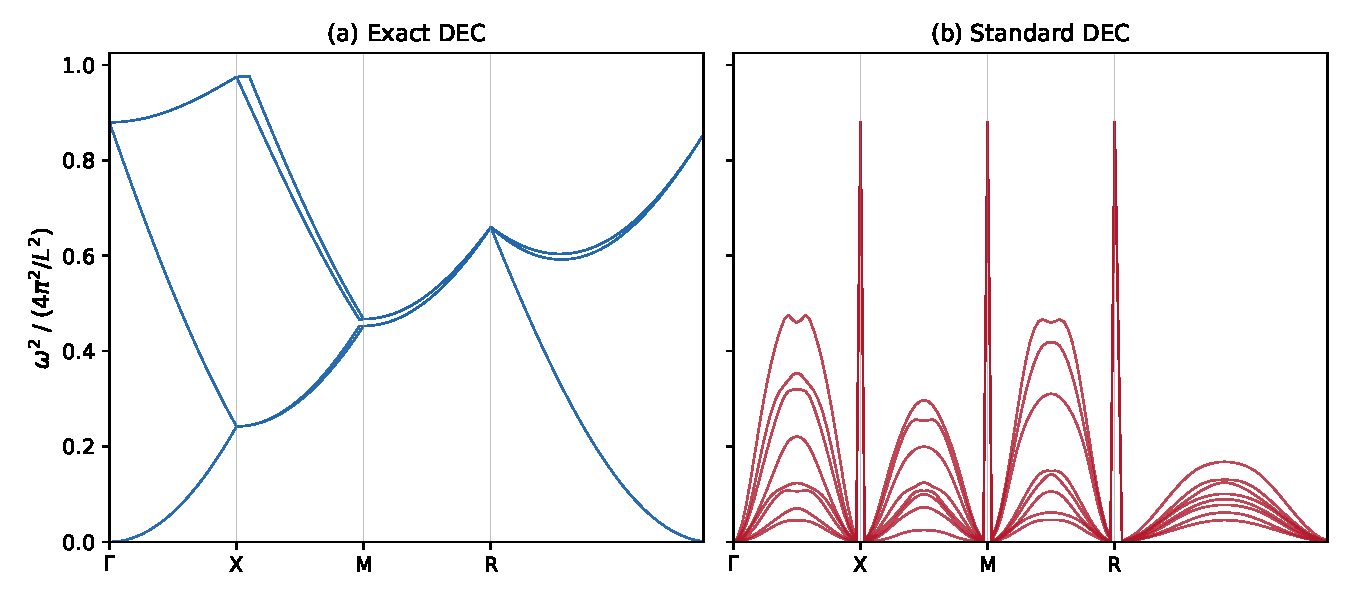
\includegraphics[width=\textwidth]{fig_bands.pdf}
\caption{Eigenvalues $\omega^2$ (normalized by $4\pi^2/L^2$) along the
high-symmetry path $\Gamma$--$X$--$M$--$R$--$\Gamma$ for the Kelvin
$N{=}2$ complex (96~vertices, 192~edges, 112~faces).
(a)~Exact construction: clean bands with twofold acoustic degeneracy.
(b)~Standard construction: spurious bands collapse toward $\omega^2 = 0$.}
\label{fig:bands}
\end{figure}

Exactness and correct kernel dimension are verified on all five structure
types, including 10 out of 10 random Voronoi seeds.

%======================================================================
\section{Application to Voronoi tessellations}\label{sec:voronoi}
%======================================================================

\begin{remark}[Voronoi optimality]\label{rem:voronoi}
On any periodic Voronoi tessellation of~$\TT^3$, the discrete metric
tensors satisfy $G = \Vol\cdot\Id$ and $H = \Vol\cdot\Id$ (where
$\Vol$ denotes the volume of the fundamental domain~$\Omega$), with
\[
G_{ij} = \sum_e (\star_1)_e\,(\boldsymbol{\ell}_e)_i\,(\boldsymbol{\ell}_e)_j,
\qquad
H_{ij} = \sum_f (\star_2)_f\,(A^f)_i\,(A^f)_j,
\]
where $\boldsymbol{\ell}_e$ is the edge direction vector (unit tangent
$\times$ length) and $A^f$ is the face area vector (unit normal $\times$
area), summed over boundary-crossing edges and faces, respectively. This
follows from the divergence theorem applied to dual cells (for~$G$) and
primal cells (for~$H$), exploiting the perpendicularity of Voronoi edges
to dual faces (details in~\cite{Toader_prep}). Verified:
$\|G/\Vol - \Id\| < 10^{-15}$ on cubic structures and
$< 5 \times 10^{-12}$ on random Voronoi (5~seeds).

Combined with Theorem~\ref{thm:main}, metric isotropy yields the exact
acoustic dispersion relation $\omega^2 = |\bk|^2 + O(|\bk|^4)$ via Schur
complement reduction of~$K(\bk)$ onto the three-dimensional harmonic
subspace at~$\Gamma$. The effective operator is proportional
to~$|\bk|^2\Id$ when $G = H = \Vol\cdot\Id$. Verified:
$c^2 \in [0.9993,\,0.9997]$ on cubic structures and
$[0.9995,\,0.9996]$ on random Voronoi seeds. On the standard complex,
$c^2$ ranges from 0.52 to~1.55.
\end{remark}

%======================================================================
\section{Conclusion}\label{sec:conclusion}
%======================================================================

The standard Bloch-periodic extension of DEC does not preserve the exact
sequence on unstructured polyhedral meshes---a structural failure, not a
numerical one. The face-boundary recurrence of Theorem~\ref{thm:main}
produces a canonical exact complex, unique up to per-face gauge, with
kernel dimension~$|V|$ and correct twisted de~Rham cohomology. Extensions
to non-flat connections (nonzero magnetic flux), non-abelian gauge groups,
and non-$\TT^3$ topologies remain open.

%======================================================================
% References
%======================================================================

\begin{thebibliography}{12}

\bibitem{Arnold2006}
D.\,N.~Arnold, R.\,S.~Falk, R.~Winther,
\emph{Finite element exterior calculus, homological techniques, and
applications},
Acta Numer.\ \textbf{15} (2006), 1--155.

\bibitem{Arnold2010}
D.\,N.~Arnold, R.\,S.~Falk, R.~Winther,
\emph{Finite element exterior calculus: from Hodge theory to numerical
stability},
Bull.\ Amer.\ Math.\ Soc.\ \textbf{47} (2010), 281--354.

\bibitem{Boffi2010}
D.~Boffi,
\emph{Finite element approximation of eigenvalue problems},
Acta Numer.\ \textbf{19} (2010), 1--120.

\bibitem{BottTu1982}
R.~Bott, L.\,W.~Tu,
\emph{Differential Forms in Algebraic Topology},
Springer, 1982.

\bibitem{Desbrun2005}
M.~Desbrun, A.\,N.~Hirani, M.~Leok, J.\,E.~Marsden,
\emph{Discrete exterior calculus},
arXiv:math/0508341, 2005.

\bibitem{DiPietro2020}
D.\,A.~Di~Pietro, J.~Droniou,
\emph{The Hybrid High-Order Method for Polytopal Meshes},
Springer, 2020.

\bibitem{Hatcher2002}
A.~Hatcher,
\emph{Algebraic Topology},
Cambridge University Press, 2002.

\bibitem{Hiptmair2002}
R.~Hiptmair,
\emph{Finite elements in computational electromagnetism},
Acta Numer.\ \textbf{11} (2002), 237--339.

\bibitem{Hirani2003}
A.\,N.~Hirani,
\emph{Discrete Exterior Calculus},
PhD thesis, Caltech, 2003.

\bibitem{Monkola2023}
S.~M\"onk\"ol\"a, J.~R\"abin\"a, T.~Rossi,
\emph{Discrete exterior calculus for photonic crystal waveguides},
Int.\ J.\ Numer.\ Methods Eng.\ \textbf{124} (2023), 1035--1054.

\bibitem{Teixeira1999}
F.\,L.~Teixeira, W.\,C.~Chew,
\emph{Lattice electromagnetic theory from a topological viewpoint},
J.\ Math.\ Phys.\ \textbf{40} (1999), 169--187.

\bibitem{Toader_prep}
A.~Toader,
\emph{Metric isotropy and spectral optimality on periodic Voronoi
tessellations},
in preparation.

\end{thebibliography}

\end{document}
